% !TEX program = xelatex
\documentclass[b5paper, 11pt, openleft]{memoir}

\usepackage{indentfirst}

%%% Font setup
\usepackage[no-math]{fontspec}
\setmainfont{Zilla Slab}
\setmonofont[Scale = MatchLowercase]{Iosevka Custom}
\XeTeXlinebreaklocale="en_EN"
\XeTeXlinebreakskip=0pt plus 3pt
\emergencystretch=1em

\usepackage{mathtools}
\usepackage[math-style = ISO, mathrm = sym, warnings-off = {mathtools-colon}]{unicode-math}
\setmathfont[Scale = MatchLowercase]{Concrete-Math.otf}
\noDisplayskipStretch
\setoperatorfont\symscr
\everymath{\displaystyle}

%%% Stylings
% Page Layout and Margins
\setsecnumdepth{subsection}
\settocdepth{subsection}
\setlrmarginsandblock{4cm}{1.5cm}{*}
\setulmarginsandblock{3cm}{2.5cm}{*}
\setlength{\headheight}{30pt}
\setlength{\parindent}{1.5cm}
\setlength{\parskip}{0.3em}
\setlength{\beforechapskip}{20pt}
\renewcommand{\arraystretch}{1}
\allowdisplaybreaks
\setSpacing{1.5}
\checkandfixthelayout

% Footnotes
\usepackage{fancyhdr}
\pagestyle{fancy}
\fancyhead[LE]{\textbf{\thepage ~ $\big\vert$ \leftmark}}
\fancyhead[RO]{\textbf{\rightmark ~ $\big\vert$ \thepage}}
\fancyhead[RE, LO, C]{}

% Styling Figures
\usepackage{multicol, caption}
\setlength{\columnseprule}{1pt}
\def\columnseprulecolor{\color{lightgray}}
\DeclareCaptionLabelSeparator{pipe}{ $\vert$ }
\captionsetup{
    labelfont = {bf},
    font = {small, sc},
    width = 0.6\textwidth,
    labelsep = pipe,
    figurename = \textbf{Fig. }
}

% Styling Titles
\renewcommand{\partnamefont}{\LARGE\bfseries\scshape\centering}
\renewcommand{\partnumfont}{\LARGE\bfseries\scshape\centering\MakeUppercase}
\renewcommand{\midpartskip}{\par\rule{1in}{0.5pt}\vspace{1em}\par}
\renewcommand{\printparttitle}{\HUGE\bfseries\scshape\centering}
\renewcommand{\afterpartskip}{\relax}
\chapterstyle{veelo}
    \renewcommand*{\printchapternum}{%
    \makebox[0pt][l]{%
    \hspace{.8em}%
    \resizebox{!}{\beforechapskip}%
    {\chapnumfont \thechapter}%
    \hspace{.8em}%
    \rule{2\midchapskip}{\beforechapskip}%
    }%
}

% Packages
\usepackage[dvipsnames]{xcolor}
\usepackage{subcaption, graphicx, pdfpages, float, wrapfig}
\usepackage{minted}
\usemintedstyle{algol_nu}
\setminted{
    frame = lines,
    bgcolor = lightgray,
    linenos,
	breaklines
}
\usepackage{csquotes}
\graphicspath{{figures/}}
\usepackage[inline]{enumitem}

\usepackage[colorlinks, allcolors = blue]{hyperref}
\usepackage{cleveref}

%%% Mathematical packages 
\usepackage[]{siunitx}
\usepackage{physics2}
\usepackage{derivative}
\usephysicsmodule{ab, ab.braket, nabla.legacy, op.legacy}
\usephysicsmodule{ab.legacy}
\usepackage[makeroom]{cancel}
% Proofs
\usepackage{amsthm}
\usepackage{tcolorbox}
\tcbuselibrary{breakable, theorems, skins}
\newtcbtheorem[auto counter, crefname = {theorem}{theorems}, Crefname = {Theorem}{Theorems}]{theorem}{Theorem}{
    coltitle = black,
    sharp corners, frame hidden, enhanced, colback = lightgray!10, breakable,
    borderline west = {3pt}{-3pt}{lightgray},
    detach title = true,
    fonttitle = \bfseries, before upper = {\tcbtitle\quad}
}{theorem}
\newtcbtheorem[auto counter, crefname = {axiom}{axioms}, Crefname = {Axiom}{Axioms}]{axiom}{Axiom}{
    sharp corners, colback = lightgray!40, colframe = darkgray, breakable
}{axiom}
\newtcbtheorem[auto counter, crefname = {definition}{definition}, Crefname = {Definition}{Definition}]{df}{Definition}{
    sharp corners, colback = lightgray!40, colframe = darkgray, breakable
}{df}
\newtcbtheorem[auto counter, number within = section]{exmp}{Example}{
    colback = lightgray!40, colframe = darkgray, breakable
}{exmp}
\newtcbtheorem[auto counter, number within = chapter, crefname = {remarks of chapter }{remarks of chapter }, Crefname = {Remarks}{Remarks}]{remark}{Remarks on chapter }{
    colback = lightgray!10, colframe = black, breakable
}{remark}

%%% Mathematical commands
% Geometry
\let\line\overline
% Mathematical constants
\newcommand{\e}{\symrm{e}}
\newcommand{\im}{\symrm{i}}
\newcommand{\cpi}{\symrm{\pi}}
\DeclareMathOperator*{\ssum}{\symrm{\Sigma}}
\DeclareMathOperator*{\Proj}{\symrm{Proj}}
\DeclareMathOperator*{\sgn}{\symrm{sgn}}
% Vector notations
\newcommand{\vv}[1]{\pmb{\symrm{#1}}}
\newcommand{\vdot}{\pmb{\cdot}}
\newcommand{\conj}{^{\ast}}
\newcommand{\dagr}{^{\dag}}
\newcommand{\trnsp}{^{\intercal}}
\newcommand{\iden}{\symbb{I}}
\newcommand{\uv}[1]{\hat{\vv{e}}_{#1}}
\newcommand{\tensor}{\otimes}
\newcommand{\bmat}[1]{
	\begin{bmatrix}
		#1
	\end{bmatrix}
}
\newcommand{\ihat}{\hat{\i}}
\newcommand{\jhat}{\hat{\j}}
\newcommand{\khat}{\hat{k}}
\newcommand{\xhat}{\hat{\vv{x}}}
\newcommand{\yhat}{\hat{\vv{y}}}
\newcommand{\zhat}{\hat{\vv{z}}}
\newcommand{\rhat}{\hat{\vv{r}}}
\newcommand{\nhat}{\hat{\vv{n}}}
\newcommand{\that}{\hat{\vv{\theta}}}
\newcommand{\phat}{\hat{\vv{\rho}}}
\newcommand{\eflux}{\symrm{\Phi}_E}
\newcommand{\mflux}{\symrm{\Phi}_B}
\newcommand{\sint}{\int_{\mathcal{S}}}
\newcommand{\aint}{\int_{\mathcal{A}}}
\newcommand{\vint}{\int_{\mathcal{V}}}
\newcommand{\cint}{\int_{\mathcal{C}}}
\newcommand{\bperm}{\symrm{\mu}_0}
\newcommand{\eperm}{\symrm{\varepsilon}_0}
\newcommand{\rc}{{{\mbox{$\resizebox{1.2ex}{1.15ex}{
\includegraphics[trim= 1em 0 14em 0,clip]{fonts/scriptr.pdf}}$}}}}
\newcommand{\brc}{{{\mbox{$\resizebox{1.2ex}{1.15ex}{
\includegraphics[trim= 1em 0 14em 0,clip]{fonts/boldcursiver.pdf}}$}}}}
\newcommand{\rchat}{{{\mbox{$\hat\rcurs$}}}}
\newcommand{\peval}[1]{\left(\left.#1\right.\right\rvert}
% Differences
\DeclareMathOperator{\kdel}{\symrm{\delta}}
\DeclareMathOperator{\ddel}{\symrm{\delta}}
\newcommand{\Dd}{\symrm{\Delta}}
% Physics quantities symbols
\newcommand{\lagr}{\mathcal{L}}
\newcommand{\haml}{\mathcal{H}}
\newcommand{\hilb}{\mathcal{E}}
\newcommand{\emf}{\mathcal{E}}
% Calculus notations
\newcommand{\appr}{\rightarrow}
\newcommand{\alc}[2][0.3]{&\parbox[c]{#1\textwidth}{#2}}
\newcommand{\pintm}[1]{\mathcal{D}[#1]}
% Mathematical conjunctions and expressions
\newcommand{\mathand}{\quad\textrm{and,}\quad}
\newcommand{\mathor}{\quad\textrm{or,}\quad}
\newcommand{\mathif}{\quad\textrm{if}\quad}
\newcommand{\mathiff}{\quad\textrm{\emph{iff}}\quad}
\newcommand{\maththerefore}{\therefore\emquad}
\newcommand{\ifft}{\emph{iff}}
% Notational commands
\newcommand{\flatfrac}[2]{#1\fracslash#2}
% Column types
\newcolumntype{C}{>{$}c<{$}}
\newcolumntype{L}{>{$}l<{$}}
\newcolumntype{R}{>{$}r<{$}}

%%% Type commands
\newcommand{\conclusion}{\section{Conclusion for Chapter \thechapter}}
\newcommand{\formula}{\section{Formula from Chapter \thechapter}}
\newcommand{\prelude}[1]{
    \chapter*{Prelude: #1}
    \addcontentsline{toc}{chapter}{Prelude: #1}
}
\newcommand{\prerequisites}[1]{\textbf{Prerequisites:}~\emph{#1}}

% Bibliographies
\usepackage[
    backend = biber,
    style = phys,
    sorting = anyvt
]{biblatex}
\addbibresource{bibfile.bib}

\usepackage[inkscapeversion = 1, inkscapelatex = true]{svg}
\svgpath{{code/}}
% Indices
% \usepackage{imakeidx}
% \makeindex

\begin{document}

\frontmatter
\title{
	\vspace{-5em}
	\textbf{
		A follow-up on "Measurement of gravity by the voltage difference induced on a solenoid by a free-falling magnet:" The flux of an actual solenoid
	}
}
\author{Puripat Thumbanthu}
\date{Started: 10/30/2024, Revision: \today}
\maketitle

\vspace{-7em}
\tableofcontents*

\mainmatter

\chapter{Introduction}

This article is a follow-up of the earlier article that I wrote as a part of a submission for the subject ESC612 (From wire to wireless), "\emph{Measurement of gravity by the voltage difference induced on a solenoid by a free-falling magnet.}" In that article, I approximated a solenoid as a simple circular loop that lies on the $x-y$ plane, and let the magnet hover at height $h$ over it. At the end, the gravitational acceleration measured was $9.52\unit{\meter\per\second}$, which is frankly better than I expected. However, I think that the $g$ value could be better if the geometry of the solenoid is actually used. Therefore, this article is going to address the magnetic flux of an actual solenoid, and compare it with the two other approximations that are commonly used.

\section{Geometries of the solenoid and its approximation}

\subsection{Geometry of an actual solenoid}

The solenoid is modeled as a helix that lies along the $z$ axis and centered at $(x, y) = (0, 0)$ shown in \cref{fig:actual-solenoid}
\begin{figure}[ht]
	\centering
	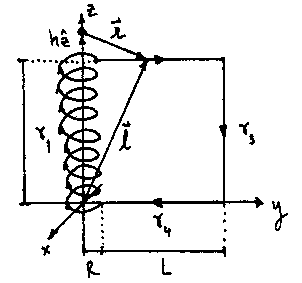
\includegraphics{solenoid.pdf}
	\caption{The solenoid's geometry}
	\label{fig:actual-solenoid}
\end{figure}

The solenoid of height $\frac{H}{2\cpi}$ that's wounded around itself $\omega$ times, where $\omega \in \mathbb{Z}$ is parameterized by the contour $\gamma$ which is given in four parts: $\gamma_1,\dots, \gamma_4$. $\gamma_1$ represents the actual solenoid, parameterized by
\begin{align}
	 & \gamma_1: \ab(x = R\sin(\omega\alpha), y = R\cos(\omega\alpha), z = \frac{H}{2\cpi}) & \alpha \in [0, 2\cpi]
\end{align}
The contour $\gamma_2$ to $\gamma_4$ represents the wire that connects the bottom of the solenoid to the top:
\begin{align}
	 & \gamma_2: \ab(x = 0, y = L\alpha + R, z = H)  & \alpha \in [0, 1] \\
	 & \gamma_3: \ab(x = 0, y = L + R, z = \alpha H) & \alpha \in [1, 0] \\
	 & \gamma_4: \ab(x = 0, y = L\alpha + R, z = 0)  & \alpha \in [1, 0]
\end{align}

\subsection{Geometry of the approximations}

Before I wrote this article, I decided asked my good friend, \emph{Nattawee Wiwatthanakul} for an opinion on how the magnetic flux may be calculated. He proposed that the solenoid's flux can be approximated with a stack of circular wires shown in \cref{fig:stacked-circles}. The wire also has radius $R$, and is stacked on itself $\omega$ times ($\omega \in \mathbb{Z}^+$), reaching the height of $H$.

\begin{figure}[ht]
	\centering
	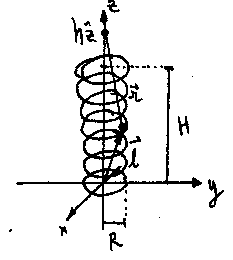
\includegraphics{stackedcircles.pdf}
	\caption{Stacked circles approximation for the solenoid}
	\label{fig:stacked-circles}
\end{figure}

Each loop contributes its own magnetic flux ${\mflux}_i$, and thus the total magnetic flux must be the sum of each loop:
\begin{equation}
	\mflux = \sum_{i = 0}^{\omega}{\mflux}_i
\end{equation}

\section{Magnetic flux}

The magnetic flux, $\mflux$ is given by
\begin{equation}
	\mflux = \sint\vv{B}\cdot\odif{\vv{a}} \label{eq:faradays-law-line-integral}
\end{equation}
where $\vv{B}$ is the magnetic field that's on the wire, and $\odif{\vv{a}}$, the area integration element. However, this cannot be done with the geometry of the solenoid because the area enclosed by the wire cannot be parameterized in a simple way. Thus, the area integral must be transformed into a line integral using the Green's theorem. Given that the vector magnetic potential $\vv{A}$ where $\vv{B} = \curl\vv{A}$, \cref{eq:faradays-law-line-integral} becomes
\begin{equation}
	\mflux = \sint\ab(\curl\vv{A})\cdot\odif{\vv{a}} = \oint_{\gamma}\vv{A}\cdot\odif{\vv{l}}.
\end{equation}
By parameterization,
\begin{equation}
	\oint_{\gamma}\vv{A}\cdot\odif{\vv{l}} = \oint\vv{A}\cdot\odv{\vv{l}}{\alpha}\odif{\alpha}
\end{equation}

\chapter{Evaluation of the magnetic flux}

\section{Magnetic flux of an actual solenoid}

\subsection{Evaluating the flux on the solenoid's contour}

The magnetic dipole is hovering at height $h$ above the middle of the solenoid. The $\vv{A}$ field of the perfect magnetic dipole is given by
\begin{equation}
	\vv{A}(\brc) = \frac{\bperm}{4\cpi}\frac{\vv{m}\times\brc}{\rc^3}. \label{eq:A-field-magnetic-dipole}
\end{equation}
We denote the vector that points from the origin to the contour as $\vv{l}$. In the solenoid's contour ($\gamma_1$),
\begin{equation}
	\vv{l} = R\sin(\omega\alpha)\xhat + R\cos(\omega\alpha)\yhat + \frac{H}{2\cpi}\alpha\zhat.
\end{equation}
Trivially,
\begin{equation}
	\odv{\vv{l}}{\alpha} = R\omega\cos(\omega\alpha)\xhat - R\omega\sin(\omega\alpha)\yhat + \frac{H}{2\cpi}\zhat. \label{eq:differential-element}
\end{equation}
Geometrically,
\begin{align}
	h\zhat + \brc & = \vv{l}                                                                                     \\
	\brc          & = \vv{l} - h\zhat                                                                            \\
	              & = R\sin(\omega\alpha)\xhat + R\cos(\omega\alpha)\yhat + \ab(\frac{H}{2\cpi}\alpha - h)\zhat,
\end{align}
and
\begin{align}
	\rc & = \sqrt{\ab(R\sin(\omega\alpha))^2 + \ab(R\cos(\omega\alpha))^2 + \ab(\frac{H}{2\cpi}\alpha - h)^2} \\
	    & = \sqrt{R^2 + \ab(\frac{H}{2\cpi}\alpha - h)^2}.
\end{align}
From \cref{eq:A-field-magnetic-dipole},
\begin{align}
	\vv{m} \times \brc & = -m\zhat \times \ab(R\sin(\omega\alpha)\xhat + R\cos(\omega\alpha)\yhat + \ab(\frac{H}{2\cpi}\alpha - h)\zhat) \\
	                   & = \begin{vmatrix}
		                       \xhat               & \yhat               & \zhat                     \\
		                       0                   & 0                   & -m                        \\
		                       R\sin(\omega\alpha) & R\cos(\omega\alpha) & \frac{H}{2\cpi}\alpha - h
	                       \end{vmatrix}                                         \\
	                   & = m\begin{vmatrix}
		                        \xhat               & \yhat               \\
		                        R\sin(\omega\alpha) & R\cos(\omega\alpha)
	                        \end{vmatrix}                                                                    \\
	                   & = mR\ab(\cos(\omega\alpha)\xhat - \sin(\omega\alpha)\yhat).
\end{align}
Therefore,
\begin{equation}
	\vv{A}(\alpha) = \frac{\bperm}{4\cpi}\frac{mR\ab(\cos(\omega\alpha)\xhat - \sin(\omega\alpha)\yhat)}{\ab(R^2 + \ab(\frac{H}{2\cpi}\alpha - h)^2)^\frac{3}{2}}
\end{equation}
And thus, from \cref{eq:differential-element}
\begin{align}
	\vv{A}\vdot\odv{\vv{l}}{\alpha} & = \begin{multlined}[t]
		                                    \frac{\bperm mR}{4\cpi}\ab(R^2 + \ab(\frac{H}{2\cpi}\alpha - h)^2)^{-\frac{3}{2}} \\
		                                    \ab(\cos(\omega\alpha)\xhat - \sin(\omega\alpha)\yhat) \vdot \ab(R\omega\cos(\omega\alpha)\xhat - R\omega\sin(\omega\alpha)\yhat + \frac{H}{2\cpi}\zhat)
	                                    \end{multlined} \nonumber \\
	                                & = \frac{\bperm mR}{4\cpi}\ab(R^2 + \ab(\frac{H}{2\cpi}\alpha - h)^2)^{-\frac{3}{2}}R\omega\ab(\cos^2(\omega\alpha) + \sin^2(\omega\alpha))                                       \\
	                                & = \frac{\bperm mR^2\omega}{4\cpi}\ab(R^2 + \ab(\frac{H}{2\cpi}\alpha - h)^2)^{-\frac{3}{2}}
\end{align}
Thus, the magnetic flux that's generated by the contour $\gamma_1$ is given by
\begin{align}
	\int_{\gamma_1}\vv{A}\vdot\odif{\vv{l}} & = \int_{0}^{2\cpi}\vv{A}\vdot\odv{\vv{l}}{\alpha}\odif{\alpha}                                                           \\
	                                        & = \int_{0}^{2\cpi}\frac{\bperm mR^2\omega}{4\cpi}\ab(R^2 + \ab(\frac{H}{2\cpi}\alpha - h)^2)^{-\frac{3}{2}}\odif{\alpha} \\
	                                        & = \frac{\mu_0 mR^2\omega}{4\cpi}\int_{0}^{2\cpi}\ab(R^2 + \ab(\frac{H}{2\cpi}\alpha - h)^2)^{-\frac{3}{2}}\odif{\alpha}
\end{align}
This integral can be easily solved by a simple substitution. Let $u = \frac{H}{2\cpi}\alpha - h$, then $\odif{u} = \frac{H}{2\cpi}\odif{\alpha}$. The bounds are changed from $\alpha = 0 \appr u = -h$, and $\alpha = 2\cpi \appr u = H - h$.
\begin{align}
	 & \frac{\mu_0 mR^2\omega}{4\cpi}\int_{0}^{2\cpi}\ab(R^2 + \ab(\frac{H}{2\cpi}\alpha - h)^2)^{-\frac{3}{2}}\odif{\alpha} \nonumber \\
	 & = \frac{\mu_0 mR^2\omega}{4\cpi}\vdot\frac{2\cpi}{H}\int_{-h}^{H - h}\ab(R^2 + u^2)^{-\frac{3}{2}}\odif{u}                      \\
	 & = \frac{\mu_0 mR^2\omega}{4\cpi}\vdot\peval{\frac{u}{R^2(R^2 + u^2)^{\frac{1}{2}}}}_{u = -h}^{u = H - h}                        \\
	 & = \frac{\mu_0 mR^2\omega}{2H}\ab(\frac{H - h}{\sqrt{R^2 + (H - h)^2}} + \frac{h}{\sqrt{R^2 + h^2}})
\end{align}

\subsection{Evaluating the flux on the solenoid's cable}

The contour $\gamma_2$ to $\gamma_4$ does not contribute to the magnetic flux. This is because the vector $\vv{m} \times \brc$ and $\vv{l}$ are orthogonal. The first one lies on the $x$ axis, but the other lies along the $y$ axis only. Therefore, the only part that contributes to the magnetic flux is $\gamma_1$:
\begin{equation}
	\mflux = \frac{\mu_0 mR^2\omega}{2H}\ab(\frac{H - h}{\sqrt{R^2 + (H - h)^2}} + \frac{h}{\sqrt{R^2 + h^2}})
\end{equation}

\section{Magnetic flux of a stacked circular wire}

Each of the loop contributes a magnetic flux $\mflux(h)$ where $h$ is the height from the center of the wire to the magnet. The contour of a circular wire at radius $R$ that's at $z = 0$ is parameterized by
\begin{equation}
	\gamma: (R\cos(\alpha), R\sin(\alpha), 0) \quad \alpha \in [0, 2\cpi]
\end{equation}
Therefore,
\begin{equation}
	\vv{l} = R\cos(\alpha)\xhat + R\sin(\alpha)\yhat,
\end{equation}
and thus,
\begin{equation}
	\odv{\vv{l}}{\alpha} = -R\sin(\alpha)\xhat + R\cos(\alpha)\yhat.
\end{equation}
Geometrically,
\begin{align}
	h\zhat + \brc & = \vv{l}                                             \\
	\brc          & = -R\sin(\alpha)\xhat + R\cos(\alpha)\yhat - h\zhat,
\end{align}
and
\begin{equation}
	\rc = \sqrt{R^2\sin^2(\alpha) + R^2\cos(\alpha) + h^2} = \sqrt{R^2 + h^2}.
\end{equation}
From \cref{eq:A-field-magnetic-dipole},
\begin{align}
	\vv{m} \times \brc & = \begin{vmatrix}
		                       \xhat         & \yhat         & \zhat \\
		                       0             & 0             & -m    \\
		                       R\cos(\alpha) & R\sin(\alpha) & -h
	                       \end{vmatrix}         \\
	                   & = m\begin{vmatrix}
		                        \xhat         & \yhat         \\
		                        R\cos(\alpha) & R\sin(\alpha)
	                        \end{vmatrix}                \\
	                   & = mR\ab(\sin(\alpha)\xhat - \cos(\alpha)\yhat);
\end{align}
therefore,
\begin{align}
	\vv{A}(\alpha) = \frac{\bperm mR}{4\cpi} \frac{\sin(\alpha)\xhat - \cos(\alpha)\yhat}{(R^2 + h^2)^{\frac{3}{2}}},
\end{align}
and
\begin{align}
	\vv{A}(\alpha)\vdot\odv{\vv{l}}{\alpha} & = \begin{multlined}[t]
		                                            \frac{\bperm mR}{4\cpi}(R^2 + h^2)^{-\frac{3}{2}} \\
		                                            \vdot \ab(\sin(\alpha)\xhat - \cos(\alpha)\yhat) \vdot \ab(-R\sin(\alpha)\xhat + R\cos(\alpha)\yhat)
	                                            \end{multlined} \\
	                                        & = \frac{\bperm mR^2}{4\cpi}(R^2 + h^2)^{-\frac{3}{2}} \ab(\sin^2(\alpha) + \cos^2(\alpha))                                                        \\
	                                        & = \frac{\bperm mR^2}{4\cpi}\frac{1}{(R^2 + h^2)^{\frac{3}{2}}}.
\end{align}
The magnetic flux of a single loop is then
\begin{align}
	\int\vv{A}(\alpha)\vdot\odv{\vv{l}}{\alpha}\odif{\alpha} & = \int_{0}^{2\cpi}\frac{\bperm mR^2}{4\cpi}\frac{1}{(R^2 + h^2)^{\frac{3}{2}}}\odif{\alpha} \\
	                                                         & = \frac{\bperm mR^2}{4\cpi}\frac{1}{(R^2 + h^2)^{\frac{3}{2}}}\int_{0}^{2\cpi}\odif{\alpha} \\
	                                                         & = \frac{\bperm mR^2}{4\cpi}(R^2 + h^2)^{-\frac{3}{2}}2\cpi                                  \\
	                                                         & = \frac{\bperm mR^2}{2}(R^2 + h^2)^{-\frac{3}{2}}.
\end{align}

In \cref{fig:stacked-circles}, the top-most loop is at $z = H$. Therefore, the distance between the magnet to each loop from the bottom-most to top-most is
\begin{equation}
	h, h - \frac{H}{\omega}, h - \frac{2H}{\omega}, \dots, h - \frac{(\omega - 1)H}{\omega}, h - H.
\end{equation}
Therefore, the total magnetic flux given by the stacked circle approximation is
\begin{align}
	\frac{\bperm mR^2}{2}\sum_{n = 0}^{\omega}\ab(h - \frac{nH}{\omega})^{-\frac{3}{2}}.
\end{align}

\input{chapters/errors}
\input{chapters/conclusion}

\printbibliography

\end{document}
